\documentclass[12pt]{report}
\usepackage{commands}

\begin{document}

\large
\begin{center}
AMSC 660 Homework 13\\
Due Dec 8\\
By Marvyn Bailly\
\end{center}
\normalsize
\hrule

%Good luck my man
%---------------%
%---Problem 1---%
%---------------%


\begin{problem}%[vskip]
\subsection*{Problem 1}

The invariant probability density for the system evolving in the double-well potential $V(x) = x^4 - 2x^2 + 1$ according to the overdamped Langevin dynamics\footnote{The overdamped Langenin stochastic differential equation is $\d X = -\nabla V(x) \d t + \sqrt{2\beta^{-1}}\d w$ where $\d W$ is the increment of the standard Brownian motion.} 3at temperature $\beta^{-1} = 1$ is given by the Gibbs pdf
\begin{equation} \label{p1}
    f(x) = \frac{1}{Z} e^{-(x^4 - 2x^2 + 1)}, ~\text{where}~ Z = \int_{-\infty}^\infty e^{-(x^4 - 2x^2 + 1)}\d x.
\end{equation}
\begin{enumerate}
    \item [(a)]
    Use the composite trapezoidal rule to find the normalization constant $Z$. Pick an interval of integration $[-a,a]$ where $a$ is large enough so that $e^{-(a^4 - 2a^2 + 1)} < 10^{-16}$.

    \item [(b)] Find the optimal value of $\sigma$ in order to use the pdf of the form
    \begin{equation*}
        g_\sigma (x) = \frac{1}{\sqrt{2 \pi \sigma^2}}e^{-x^2/(2\sigma^2)},
    \end{equation*}
    for sampling RV with pdf $f(x)$ (\fullref{p1}) by means of the acceptance-rejection method. The optimal $\sigma$ minimizes the constant $c$. 

    \noindent
    \textit{Hint: first find analytically}
    \begin{equation*}
        x^* = \text{argmax}_{x \in \R} \frac{f(x)}{g_\sigma(x)}
    \end{equation*}
    \textit{as a function of $\sigma$. Then you can find the optimal $\sigma$ using e.g. the function} \verb+fminbnd+ \textit{in MATLAB.}

    \item [(c)]  Sample RV $\eta$ with pdf $f (x)$ (\fullref{p1}) using the acceptance-rejection method. Check that the ratio of the total number of samples and the number of accepted samples is close to $c$. Plot a properly scaled histogram for the obtained samples and compare it with the exact distribution (with $Z$ found numerically). An example of generating such a histogram is given in the code in Section 3.3 in
    MonteCarloAMSC660.pdf.
    
    \noindent
    \textit{Hint: to generate samples of $\mathcal{N}(0,\sigma^2)$, generate samples from $\mathcal{N}(0,1)$ and multiple by $\sigma$}

    \item [(d)] 
    Find $E[|x|]$ for the pdf $f(x)$ using the Monte Carlo integration.



\end{enumerate}


\subsection*{Solution}
\begin{proof}

Consider the invariant probability density for the system evolving in the double-well potential $V(x) = x^4 - 2x^2 + 1$ which has pdf
\begin{equation}\label{p1eq}
    f(x) = \frac{1}{Z} e^{-(x^4 - 2x^2 + 1)}, ~\text{where}~ Z = \int_{-\infty}^\infty e^{-(x^4 - 2x^2 + 1)}\d x.
\end{equation}
\begin{enumerate}
    \item [(a)]
    We wish to use the composite trapezoidal rule to find the normalization constant $Z$. We will use an interval of integration $[-a,a]$ where $a$ is large enough so that $e^{-(a^4-2a^2 + 1)} < 10^{-16}$. Recall that trapezoidal rule over $[a,b]$ is of the form
    \begin{equation*}
        Z = \int_{a}^{b} f(x) \d x = \frac{\Delta x}{2}\paren{f(a) + 2\sum_{k=1}^{N-1} \paren{f(a + k\Delta x)} + f(b)}, 
    \end{equation*}
    where $\Delta x = \frac{b-a}{N}$ where $N$ is the number of sub-intervals being used. Thus we find that
    \begin{equation*}
        Z \approx \frac{a}{N}\paren{e^{-V(-a)} + 2\sum_{k=1}^{N-1} \paren{e^{-V\paren{-a + \frac{2ka}{N}}}} + e^{-V(a)}},
    \end{equation*}
    and using the following code we find $a = 3$ to be a suitable value and using $N = 500$ we find that $z \approx 1.97$.

    \begin{lstlisting}[style=Matlab-editor]
trapezoid(@(x)(exp(-(x^4 - 2*x^2 + 1))),-3,3,500)

function sol = trapezoid(fun,a,b,N)
    sol = 0;
    dx = (b-a)/N;
    approx = 0;
    for i = 0:N
        if i == 0 || i == N
            approx = fun(a);
        else
            approx = 2*fun(a + i*dx);
        end
        sol = sol + approx;
    end
    sol = dx/2 * sol;
end
    \end{lstlisting}

    \item [(b)]
    Next, we wish to find the optimal value of $\sigma$ in order to use the pdf of the form
    \begin{equation*}
        g_\sigma = \frac{1}{\sqrt{2\pi \sigma^2}}e^{-x^2/(2\sigma^2)},
    \end{equation*}
    for sampling random variables with pdf given by \fullref{p1eq}. We begin by finding
    \begin{align*}
        x^*(\sigma) &= \text{argmax}_{x \in \R} \frac{f(x)}{g_\sigma(x)}\\
        &=  \text{argmax}_{x \in \R} \frac{\frac{1}{Z} e^{-(x^4 - 2x^2 + 1)}}{\frac{1}{\sqrt{2\pi \sigma^2}}e^{-x^2/(2\sigma^2)}}\\
        &=  \text{argmax}_{x \in \R} \frac{ \sqrt{2\pi \sigma^2 }e^{x^2/(2\sigma^2)-(x^4 - 2x^2 + 1)}}{Z},
    \end{align*}
    Now we can find the max $x$ by setting the derivative equal to zero. Observe
    \begin{align*}
        \dd{}{x} \sqrt{\frac{\pi }{2}} \sqrt{\sigma ^2} e^{-x^4+\frac{x^2}{2 \sigma ^2}+2 x^2-1} &= \sqrt{\frac{\pi }{2}} \sqrt{\sigma ^2} e^{-x^4+\frac{x^2}{2 \sigma ^2}+2 x^2-1} \left(-4 x^3+\frac{x}{\sigma ^2}+4 x\right) = 0,
    \end{align*}
    and solving we find that
    \begin{equation*}
        x = 0 \and x = \pm \sqrt{1 + (2\sigma)^{-1}}.
    \end{equation*}
    To find the max, we plot $\ddn{2}{}{x}x^*(\sigma)$ using the three values to find $x_{\text{max}} = \sqrt{1 + (2\sigma)^{-1}}$ achieves the maximum, as seen in Figure \ref{figmax} since CP3 which corresponds $x_{\text{max}}$ is negative. Thus we have found
    \begin{equation*}
        x^*(\sigma) = \sqrt{\frac{\pi }{2}} \sqrt{\sigma ^2} \exp \left(\frac{4 \sigma ^2+1}{2 \sigma ^2}-\frac{\left(4 \sigma ^2+1\right)^2}{16 \sigma ^4}+\frac{4 \sigma ^2+1}{8 \sigma ^4}-1\right).
    \end{equation*}
    Now using MATLAB's \verb+fminbnd+ function on $x^*(\sigma)$ we find the optimal sigma to be $\sigma = 1.098699$. Finally we can compute $c = 2.203908$.
    \begin{figure}[H]
        \centering
        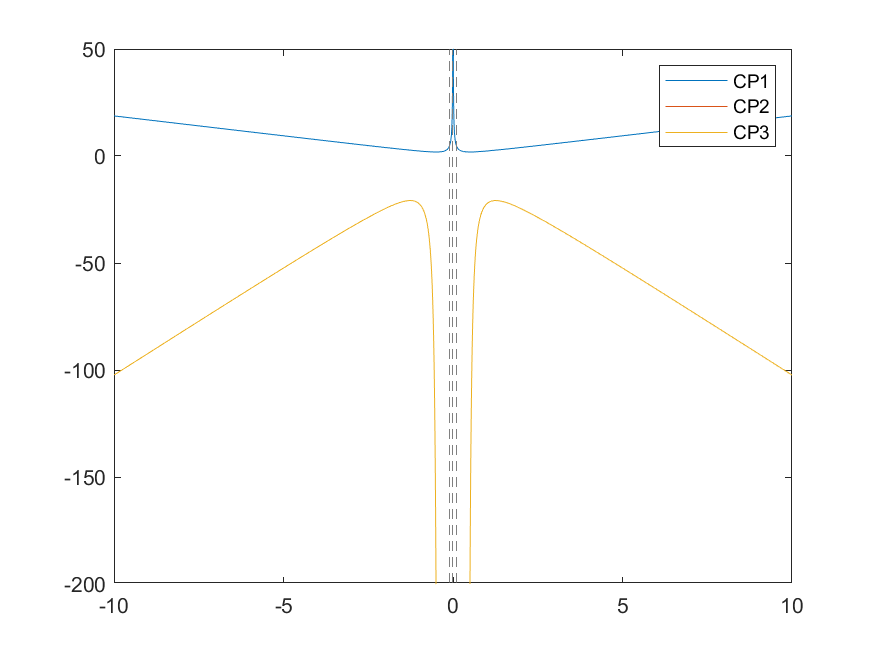
\includegraphics[width=0.7\textwidth,height=\textwidth,keepaspectratio]{images/q1max.png}
        \caption{Plot of the $\ddn{2}{}{x}x^*(\sigma)$ where the three different critical points are used. CP1 corresponds to $0$, CP2 with $-\sqrt{1+(2\sigma)^{-1}}$, and CP3 with $\sqrt{1+(2\sigma)^{-1}}$}. 
        \label{figmax}
    \end{figure}
    
    \item [(c)]
    Next. we wish to sample the random variable $\eta$ with pdf $f(x)$ using the acceptance-rejection method and our previously found $Z$ value. Implementing the acceptance-rejection method, as shown below, and using $10^8$ samples, we generate $\eta$. We can compute the ratio of the total number of samples and the number of accepted samples to be $2.203885$ which is close to the previously found $c = 2.203908$ as expected. We can also plot the histogram for the obtained samples and compare it with the exact distribution as seen in Figure \ref{fighisto}. 

    \begin{lstlisting}[style=Matlab-editor]
function eta = acceptReject(c,sigma,f,g)
    N = 1e8; % the number of samples
    v = randn(N,1);
    xi = sigma*v;
    u = rand(N,1);

    ind = find(u <= f(xi) ./ (c * g(xi)));
    Na = length(ind); % the number of accepted RVs
    eta = xi(ind);
    fprintf("N/Na = %d\n",N/Na);
end
    \end{lstlisting}
    
    \begin{figure}[H]
        \centering
        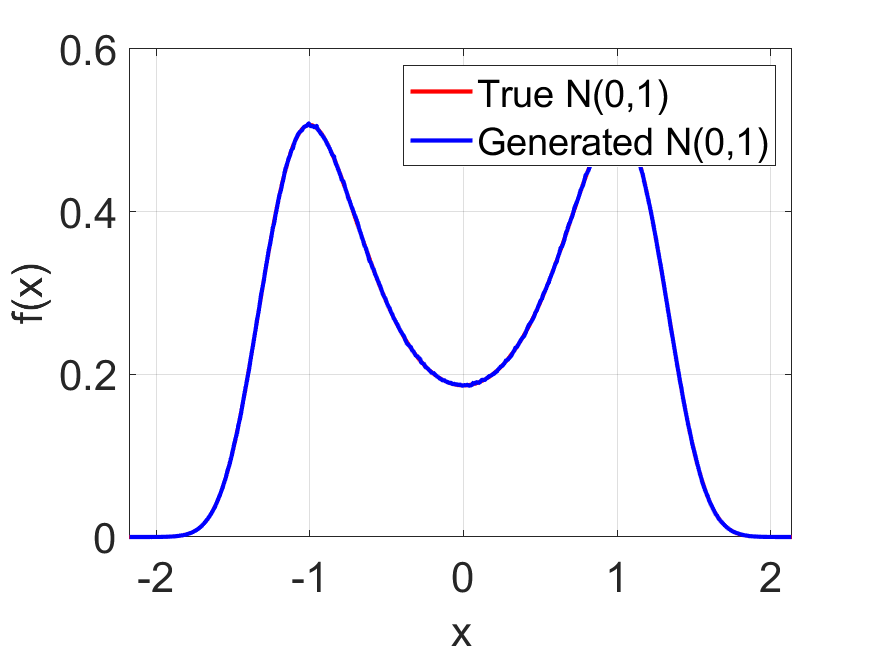
\includegraphics[width=0.7\textwidth,height=\textwidth,keepaspectratio]{images/q1histo.png}
        \caption{Histogram for the obtained samples (seen in blue) compared with the exact distribution (seen in red).}
        \label{fighisto}
    \end{figure}

    \item [(d)]
    Finally we can use the previously generated samples $\eta$ to compute $E[|x|]$ for the pdf $f(x)$ using Monte Carlo Integration
    \begin{equation*}
        \mathbb{E}_{f}[|x|] \approx \frac{1}{n}\sum_{i=1}^n |\eta_i| = 0.827411.
    \end{equation*}
\end{enumerate}

\noindent
Complete code can be found at \url{https://github.com/MarvynBailly/AMSC660/tree/main/homework13}

\end{proof}
\end{problem}




%---------------%
%---Problem 2---%
%---------------%


\begin{problem}%[vskip]
\subsection*{Problem 2}

The unit cube in $\R^d$ centered at the origin is the set
\begin{equation*}
    C^d = \brac{x \in \R^d | \max_{1 \leq i \leq d} |x_i| \leq \frac{1}{2}},
\end{equation*}
while the unit ball in $\R^d$ centered at the origin is the set
\begin{equation*}
    B^d = \brac{x \in \R^d | \sum_{i=1}^d x_i^2 \leq 1}.
\end{equation*}
Obviously, all centers of the $(d-1)$-dimensional faces of $C^d$, i.e., the points with one coordinate $\pm \frac{1}{2}$ and the rest zeros, lie inside $B^d$. The most remote points of $C^d$ from the origin are the corners with all coordinates $\pm \frac{1}{2}$. The distance of the corner of $C^d$ from the origin is $\sqrt{d}/2$. For $d \geq 5$, the corners of $C^d$ and some their neighborhoods lie outside $B^d$. The $d$-dimensional volume of $C^d$ is $1$, while the volume of the $d$-dimensional unit ball $B^d$ tends to zero as $d \to \infty$:
\begin{equation*}
    \text{Vol}(C^d) = 1, \quad \text{Vol}(B^d) = \frac{\pi^{d/2}}{\frac{d}{2}\Gamma\paren{\frac{d}{2}}} \to 0 ~\text{as}~ d\to \infty.
\end{equation*}
Therefore, the fraction of the unit cube $D^c$ lying inside $B^d$ also tends to zero as $d \to \infty$. You can read about this phenomenon in [1].

\noindent
\textbf{Task.} Calculate $\text{Vol}(B^d \cap C^d)$ in $d = 5,10,15,20$ using Monte Carlo integration in two ways
\begin{enumerate}
    \item [(a)] Use a sequence of independent uniformly distributed random variables in the unit cube $C^d$.
    \item [(b)] Use a sequence of independent uniformly distributed random variables in the unit ball $B^d$. (You need to think of a way to generate such a random variable.)
\end{enumerate}

\subsection*{Solution}
\begin{proof}

Consider the unit cube in $\R^d$ centered at the origin given by
\begin{equation*}
    C^d = \brac{x \in \R^d | \max_{i \leq i \leq d}|x_i \leq \frac{1}{2}},
\end{equation*}
and the unit ball in $\R^d$ centered at the origin given by
\begin{equation*}
    B^d = \brac{x \in \R^d | \sum_{i =1}^d x_i^2 \leq 1}.
\end{equation*}
Note that the volume of $C^d \and B^d$ are given by
\begin{equation*}
    \text{Vol}(C^d) = 1, \quad \text{Vol}(B^d) = \frac{\pi^{d/2}}{\frac{d}{2}\Gamma\paren{\frac{d}{2}}} \to 0 ~\text{as}~ d\to \infty.
\end{equation*}
We wish to calculate $\text{Vol}(B^d \cap C^d)$ in $d = 5,10,15,20$ using Monte Carlo integration in two ways:
\begin{enumerate}
    \item [(a)] 
    We first wish to use a sequence of independent uniformly distributed random variables in the unit cube $C^d$. We can generate these points in MATLAB using 
    \begin{verbatim}
        xi = rand(N, d) - 0.5;
    \end{verbatim}
    which generates $N$ uniformly distributed random variables in $\R^d$ and centers them about the origin by subtracting $\frac{1}{2}$. Next, we can check how many of these points lie within $B^d$ by checking 
    \begin{verbatim}
        ind = find(sum(xi.^2, 2) <= 1)
    \end{verbatim}
    Finally, we find the volume of $B^d \cap C^d$ by computing the ratio of points outside and within $B^d$ and scaling it by the volume of $C^d$ which is $1$. Putting this all together, we get the following algorithm:
    \begin{lstlisting}[style=Matlab-editor]
function vol = estimateVolumeCubeIntersectionBall(d, numSamples)
    xi = rand(numSamples, d) - 0.5;
    
    ind = find(sum(xi.^2, 2) <= 1); %see if it's in the B^d
    Na = length(ind); 

    vol = Na / numSamples; % Volume of B^d \cap C^d
end
    \end{lstlisting}  


    \item [(b)] Next we wish to use a sequence of independent uniformly distribution random variables in $B^d$. To generate these random variables, we begin by generating uniformly distributed random variable $\xi$ between $0$ and $1$. Next, we scale the random variable to lie on the surface of the unit ball by normalizing to have a radius of $1$. To place the points uniformly within the unit ball, we multiply by the $d^\text{th}$ root of a random variable which is uniformly distributed between $0$ and $1$. With the random variables, we can find the volume of $B^d \cap C^d$ by finding the ratio of points that lie within and without $C^d$ and multiplying by the volume of $B^d$. This gives the following algorithm
    \begin{lstlisting}[style=Matlab-editor]
function vol = estimateVolumeBallIntersectionCube(d, n)
    xi = randn(n, d);
    radii = sqrt(sum(xi.^2, 2))*ones(1,d);

    % Scale points to be uniformly inside the ball
    scale = rand(n, 1).^(1/d) * ones(1,d);
    xi = (xi .* scale) ./ (radii);

    % Check if points are inside the unit cube
    ind  = find(max(abs(xi),[],2) <= 0.5);
    Na = length(ind);
    
    % Calculate the fraction of points inside the cube
    fractionInside = Na / n;

    % Volume of the d-dimensional unit ball
    ballVolume = pi^(d / 2) / (d / 2  * gamma(d / 2 ));
    
    % Approximate volume of the intersection
    vol = fractionInside * ballVolume;
end  
    \end{lstlisting} 
\end{enumerate}
Running the code for $d = 5,10,15,20$ using $10^{5}$ samples, results are shown in Table \ref{TABLLEEEE}, we see that the volume tends to zero as $d \to \infty$. This is expected since $\text{Vol}(B^d) \to 0$ as $d \to \infty$. 


\begin{table}[h!]
    \centering
    \begin{tabular}{c|c|c}
        Volume of $C^d \cap B^d$&  method a& method b \\ \hline
        $d = 5$&  .9995700 &  1.002089 \\
        $d = 10$&  .7622900 & .7624302  \\
        $d = 15$&  .1997000 &  .1972851 \\
        $d = 20$& .01769000 &  .01822563
    \end{tabular}
    \caption{}
    \label{TABLLEEEE}
\end{table}





\noindent
Complete code can be found at \url{https://github.com/MarvynBailly/AMSC660/tree/main/homework13}



\end{proof}
\end{problem}




\end{document}